\documentclass{article}
\usepackage{tikz}
\usetikzlibrary{positioning,fit}

\begin{document}

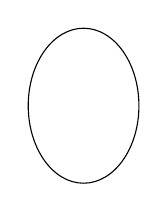
\begin{tikzpicture}
\draw (0,0) ellipse(20pt and 28pt);
\end{tikzpicture} \\

\tikz \draw (0,0) circle(4ex);\\
\tikz \draw[line width=2mm] (0,0)
circle(4ex);\\

\begin{tikzpicture}
  \draw[step=.25mm,gray,thick] (-1,-1) grid (1,1);
\end{tikzpicture}
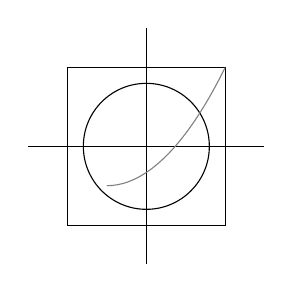
\begin{tikzpicture}
   \draw(-1.5,0)--(1.5,0);\draw(0,-1.5)--(0,1.5);\draw (0,0) circle(.8cm);\draw(-1,-1)rectangle(1,1);\draw[gray](-.5,-.5) parabola (1,1);
\end{tikzpicture}
\begin{tikzpicture}
  \draw(-.5,0)--(1.5,0);
  \draw(0,-.5)--(0,1.5);
  \draw(1,0) arc(-25:70:1cm);
\end{tikzpicture}
\tikz\draw (0,0) arc (0:180:1cm);
\tikz \draw[fill=gray!50] (4,0)--+(30:1cm) arc (30:60:1cm) -- cycle;

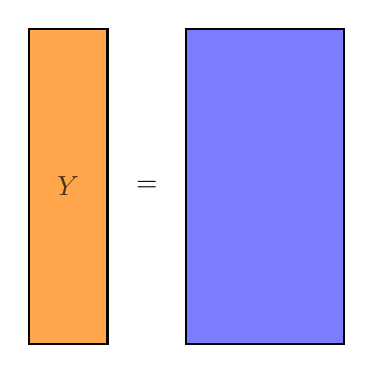
\begin{tikzpicture}
\node (rect) at (0,0) [draw,thick,fill=orange,fill opacity=0.7,minimum width=1cm,minimum height=4cm] {$Y$};
%方法一 \node一个通用的命令,可以在后面的[]中画任何预先定义好的形状。(rect)是给这个node取的名字,draw是指边框,thick是指边框的粗细。fill=orange是指在这个边框围起来的部分填入橙色,fill opacity是指橙色透明度如何,width和height是长宽;前面有minimum表示如果后面{}中的公式占空间太大的画,矩形可以自动改变大小。
\node at (1,0){$=$};
\draw[thick] (1.5,-2)rectangle(3.5,2);
\fill[blue,opacity=0.3](1.5,-2)rectangle(3.5,2);
%方法二 手动 \draw命令指定从(1.5,-2)到(3.5,2)画一个矩形,后面的\fill命令来决定填什么颜色。
\draw[thick,fill=blue,fill opacity=0.3]
(1.5,-2)--(1.5,2)--(3.5,2)--(3.5,-2)--cycle;
\end{tikzpicture};
% 和方法二同样在一个地方画矩形;只是这次人工指定了每个顶点的位置;最后的--cycle和--(1.5,-2)是等价的;而且填色的部分是直接作为\draw命令的选项来设置的。
%\begin{tikzpicture}
%\node at (2.5,0){$\Psi$}
%\tikzstyle{greenrect}=[rectangle,draw,fill=green!50,fit=#1];
%\coordinate(A) at (4,1);
%\coordinate(B) at (5,-1);
%\node[greenrect={(A) (B)}]{};
%\node at (4.5,0){$\beta$};
%\end{tikzpicture}
% 方法三使用了TikZ的fit库。


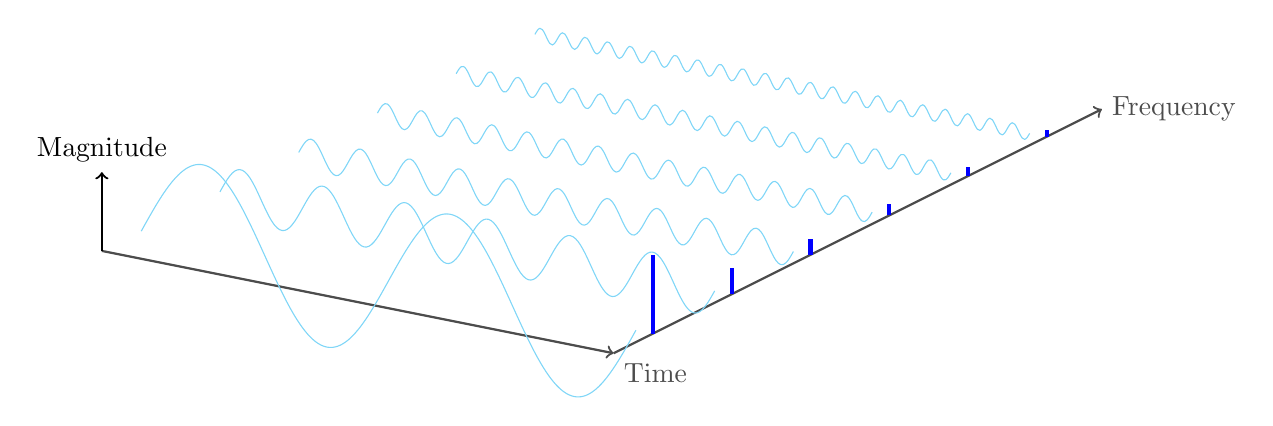
\begin{tikzpicture}
[x={(1cm,0.5cm)},z={(0cm,0.5cm)},y={(1cm,-0.2cm)}]
\draw[->,thick,black!70](0,6.5,0)--(6.2,6.5,0) node[right]{Frequency}; %频率轴
\draw[->,thick,black!70](0,0,0)--(0,6.5,0) node[below right] {Time}; %时间轴
\draw[->,thick](0,0,0)--(0,0,2) node[above]{Magnitude};
\foreach \n in {0.5,1.5,...,5.5}{
\draw [cyan!50,domain=0:2*pi,samples=200,smooth]
plot(\n,\x,{sin(4*\n*\x r)/\n});
\draw[blue,ultra thick](\n,6.5,0)--(\n,6.5,1/\n);
}
%频率逐渐增大振幅逐渐变小的正弦函数
\end{tikzpicture}

\end{document}
